\documentclass[a4paper, 12pt]{article}

\usepackage[utf8]{inputenc}
\usepackage[T2A]{fontenc}
\usepackage[english, russian]{babel}

\usepackage{cmap}
\usepackage{calc}
\usepackage{enumitem}
\setlist{nolistsep}
\usepackage{mathtext,mathtools,amsmath}
\usepackage{xcolor}
\definecolor{allrefs}{HTML}{1010aa}
\usepackage[
	linktoc=page,
	colorlinks=true,
	allcolors=allrefs
]{hyperref}

\frenchspacing
\linespread{1.3}
\usepackage{indentfirst}
\usepackage{graphicx}
\usepackage[multidot]{grffile}
\usepackage[labelsep=period]{caption}
\makeatletter
\g@addto@macro\@floatboxreset\centering
\makeatother

\usepackage[
	hmargin=1in,
	vmargin=1in
]{geometry}

\def\d{\,\mathrm{d}}
\def\vec#1{\mathbf{#1}}
\def\L{\mathcal{L}}
\def\phi{\varphi}

%note Bibliography styling 
\def\bibauthor#1{#1} % normal text, not italic
\def\bibtitle#1{\textit{#1}} % italic titles




%%%%%%%%%%%%%%%%%%%%%
%% Document begins %%
%%%%%%%%%%%%%%%%%%%%%
\begin{document}

\begin{center}
\bf\LARGE
Физический вакуум. Эффект Казимира
\end{center}
\tableofcontents

%note \setcounter is only for this template document, not for the final book 
\setcounter{section}{6}
\section{Физический вакуум. Эффект Казимира}

%%%%%%%%%%%%%%%%%%%%%%%%%%%%%%%%%%%%%%%%%%%%%%%%
\subsection{Теория поля и квантовая теория поля}
Для упрощения восприятия многих вопросов, упоминаемых в данном тексте, будет полезно иметь некоторое представление об объектах, с которыми придется работать во избежание принципиально ошибочных интерпретаций. 
Стартовать с нуля невозможно, поэтому предполагается, что читатель знаком с классической теоретической физикой и нерелятивистской квантовой механикой. 

В теоретической физике основными инструментами были лагранжиан, который для системы с $n$ степенями свободы зависел от $n$ обобщенных координат и их производных по времени $L = L(q_1, \ldots, q_n, \dot{q}_1, \ldots, \dot{q}_n)$, и интеграл по времени от него -- действие $S = \int L\d t$. 
Из принципа наименьшего действия получались уравнения эволюции системы
\begin{equation}
\frac{\d}{\d t} \left(\frac{\partial L}{\partial \dot{q_i}}\right) - \frac{\partial L}{\partial q_i} = 0 ,
\quad
i = \overline{1,n}
.
\label{eq:q.evolution}
\end{equation}
Классическая теория поля, условно говоря, представляет собой переход к бесконечному числу степеней свободы, когда набор обобщенных координат $q_i$ заменяется на поле $\phi(\vec{x}, t)$, где $\vec{x}$~-- радиус-вектор, а их производные по времени $\dot{q}_i$~-- на частные производные поля по всем переменным. 
Вместо лагранжиана $L$ в этом случае удобно рассматривать его плотность $\L$. 
Тогда действие принимает вид 
$$
S = \int L(\phi, \partial\phi) \d t = \int \L(\phi, \partial\phi) \d^3 \vec{x} \d t = \int \L(\phi, \partial\phi) \d^4x,
$$
где $x$ -- четырехвектор в пространстве-времени. 
Принцип наименьшего действия приводит к уравнению
\begin{equation}
\sum\limits_{\mu=0}^{3}\frac{\partial}{\partial x^\mu} \left(\frac{\partial \L}{\partial \left(\frac{\partial \phi}{\partial x^\mu}\right)}\right) - \frac{\partial \L}{\partial\phi} = 0 ,
\label{eq:phi.evolution}
\end{equation}
очень похожему на~(\ref{eq:q.evolution}), но в явном виде инвариантному относительно преобразований Лоренца.
Как видно из приведенных формул, смысл разделять время и пространство полностью пропадает, теория становится более приспособленной к релятивистскому рассмотрению. 

Теперь, осуществляя переход к квантовой теории, как это было с квантовой механикой, все величины нужно заменить соответствующими операторами. 
Выходит, что лагранжиан сам по себе зависит от операторов, и по ним придется дифференцировать. 
К тому же, уравнения эволюции системы, аналогичные~(\ref{eq:phi.evolution}), содержат теперь только операторы. 
Это, на первый взгляд, порождает довольно сложную интерпретацию любых процедур и результатов, однако на помощь приходят теория возмущений и диаграммы Фейнмана. 
Последовательно примененные операторы $\phi(x_i)\,\phi(x_{i-1})\ldots\phi(x_1)$, усредненные по квантовому состоянию, будут выражать амплитуду вероятности прохождения частицы через точки $x_1, \ldots, x_i$.

Единственным объектом, определяющим свойства полей, а с ними и частиц, является лагранжиан. 
Все характеристики процессов, включая константы взаимодействия и массы частиц, будут определяться его формой. 
Осознавая это, гораздо проще воспринимать изменения этих параметров в различных ситуациях. 

%%%%%%%%%%%%%%%%%%%%%%%%%%%%%%%%
\subsection{Виртуальные частицы}

В квантовой теории поля точное решение существует лишь для небольшого набора модельных гамильтонианов, которые зачастую далеки от нужных для описания эксперимента. 
Однако, относительно простой задачей является рассмотрение ни с чем не взаимодействующего поля. 
Если имеется решение для этого случая и если взаимодействие не слишком велико, полноценный гамильтониан всех необходимых полей с учетом их взаимодействия можно представить в виде суммы гамильтониана невзаимодействующих полей и гамильтониана взаимодействия, который из-за малости можно рассматривать как возмущение. 
Тогда можно решать задачу, применяя теорию возмущений. 

\begin{figure}
\includegraphics[width=.45\linewidth]{figs/VirGamma}
\caption{Пример виртуальной частицы в диаграмме Фейнмана.}
\label{fig:VirGamma}
\end{figure}

В этом случае квантовая теория поля допускает интерпретацию взаимодействия частиц как обмена виртуальной частицей (или несколькими). 
Виртуальной называется частица, которая и рождается, и умирает в пределах одной диаграммы Фейнмана, например, как $\gamma$-квант на рис.~\ref{fig:VirGamma}. 

Многие квантовые числа виртуальных частиц могут не совпадать с привычными нам. 
Например, виртуальный $\gamma$-квант может иметь продольную поляризацию, отличный от единицы спин, ненулевой или даже отрицательный квадрат четырехимпульса $p^2$, который для реальных частиц равен квадрату массы. 
Никакие характеристики виртуальных частиц нельзя измерить физическими приборами, об их существовании можно судить лишь по согласию эксперимента и основанных на их участии в реакции расчетах. 
Вероятность возникновения виртуальных частиц зависит от величины константы взаимодействия, из-за которого они возникли, и их импульса. 
Например, амплитуда вероятности может содержать множитель 
$$ \frac{1}{p^2 - m^2}, $$
где $p$ -- четырехимпульс виртуальной частицы, а $m$ -- масса реальной. 


%%%%%%%%%%%%%%%%%%%%%%%%%%%%%%%
\subsection{Содержимое вакуума}

В отличие от классической физики, в квантовой теории допускается случай, когда единственная частица и испускает, и поглощает виртуальный квант поля (однако это не означает, что частица может действовать на саму себя). 
И, что еще важнее, если гамильтониан содержит, например, поле фермионов, поле бозонов и их взаимодействие, то даже в основном состоянии (вакууме) получающейся системы могут возникать виртуальные пары частица-античастица. 
Подобные ситуации обусловлены присутствием квантовых полей даже в вакууме.

\begin{figure}[b]
\includegraphics[width=.45\linewidth]{figs/Gamma-ee}
\caption{Превращение виртуального фотона в электрон-позитронную пару.}
\label{fig:gamma-to-ee}
\end{figure}

Для начала обсудим немного более простой случай -- взаимодействие двух заряженных частиц.
Для иллюстрации будем считать, что все возможные заряженные частицы -- электроны и позитроны. 
Простейший случай обмена виртуальным фотоном изображен на рис.~\ref{fig:VirGamma}. 
Такой прямой обмен не приводит ни к каким неожиданным явлениям и поэтому не представляет особого интереса. 
Одно из возможных усложнений -- превращение виртуального фотона ``по пути'' в электрон-позитронную пару, как показано на рис.~\ref{fig:gamma-to-ee}. 
В этом случае виртуальный фотон часть времени проводит в виде электрон-позитронной пары, что влияет на результирующий эффективный потенциал, который ощущают обе взаимодействующие частицы. 
Учет диаграмм такого типа приводит к, на первый взгляд, неожиданным последствиям -- видимый заряд частиц уменьшается. 

\begin{figure}
\includegraphics[width=.6\linewidth]{figs/VacPol}
\caption{Поляризация вакуума вокруг заряженной частицы и экранировка ее истинного заряда.}
\label{fig:VacPol}
\end{figure}

Осознать результат можно следующим образом. 
Так как виртуальный фотон может превратиться в электрон-позитронную пару в какой угодно точке, можно считать, что пространство заполнено множеством электрон-позитронных пар, которые в каком-то приближении являются маленькими диполями. 
Поскольку, например, электрон, имеет отрицательный заряд, эти диполи будут ориентированы положительной стороной к нему, пространство вокруг электрона будет иметь поляризацию и станет экранировать настоящий заряд, как показано на рис.~\ref{fig:VacPol}. 
Это явление известно как поляризация вакуума. 

Возникновение виртуальных частиц в вакууме выглядит примерно так же. 
Рождающиеся частицы либо сами взаимодействуют с чем-то, либо рождают другие. 
Этот процесс называют квантовыми флуктуациями. 
В результате них, когда реальная частица попадает в какую-то область пространства, она не существует одна, а становится окружена множеством виртуальных, которые из-за наличия взаимодействия с реальной перераспределяются, как это делали электрон-позитронные пары, и изменяют видимые характеристики частицы. 
Так происходит, например, с магнитным моментом. 
Спиновый магнитный момент свободного электрона не равен $\mu_B$, то есть спиновый фактор Ланде $g_s$ не равен в точности $2$, в отличие от предсказаний теории Дирака. Влияние на него оказывают виртуальные частицы вакуума и диаграммы, подобные изображенной на рис.~\ref{fig:g_s}, поскольку они как бы ``размывают'' электрон в пространстве. 
Относительное отличие фактора Ланде электрона от двойки $a_e = \frac{g_s - 2}{2}$ является одним из наиболее точных результатов, подтверждающих квантовую теорию поля. 
Теория и эксперимент согласуются вплоть до 12-го порядка~\cite{electron.g-2.exp, electron.g-2.theory}
\begin{align*}
a_e^\text{теор.} &= 0.001\,159\,652\,181\,643\ (763), \\
a_e^\text{эксп.} &= 0.001\,159\,652\,180\,73\ (28). 
\end{align*}

\begin{figure}
\includegraphics[width=.25\linewidth]{figs/Magnetic-anom-e}
\caption{Простейшая диаграмма, дающая вклад в аномальный магнитный момент фермионов.}
\label{fig:g_s}
\end{figure}

Еще одно экспериментальное подтверждение теории связано со спектром атома водорода. 
Как известно, уровни энергии в этой системе с учетом спина электрона зависят от главного квантового числа $n$ и полного момента электрона $j$, но не от его орбитального момента $l$. 
Это случайное вырождение по $l$ обусловлено не симметрией потенциала, а показателем степенной зависимости его от расстояния между частицами ($U_\text{кул} \sim 1/r$).
И это вырождение снимается при учете нескольких явлений квантовой электродинамики. 
Впервые зависимость энергии от орбитального момента электрона была экспериментально обнаружена для уровней $2s_{1/2}$, $2p_{1/2}$ Лэмбом и Ризерфордом~\cite{LambShift.exp}, а смещение этих уровней в спектре было названо лэмбовским сдвигом. 
%
Теория объясняет это следующим образом.
Из-за поляризации вакуума потенциал кулоновского взаимодействия точечных частиц имеет близкое к дельта-функции слагаемое при нулевом расстоянии между ними. 
Оно приводит к смещению $S$ уровней, поскольку для них $\psi(\vec{x}=0)\neq0$. 
Однако, учет неточечности протона осложняет ситуацию и уменьшает конечный вклад, в итоге эта часть смещения довольно мала. 
Большее влияние оказывает взаимодействие электрона с квантовыми флуктуациями вакуума. 
Их можно приблизительно считать малыми колебаниями электрона, которые в его собственной системе отсчета (которая с достаточной точностью близка к инерциальной) видны как малые колебания ядра, и поэтому тоже дают вклад только в $S$ уровни электрона. 
Изучение лэмбовского сдвига важно, поскольку он связан в основном с квантовыми флуктуациями, поведение которых представляет большой интерес. 
Для примера их важности достаточно упомянуть излучение частиц черными дырами, предложенное Стивеном Хокингом~\cite{Hawking}.

%%%%%%%%%%%%%%%%%%%%%%%%%%%%%%%%%%%%%%%%%%%
\subsection{Вакуум сильного взаимодействия}

\begin{figure}[b]
\null
\hfill
\includegraphics[width=.45\linewidth]{figs/Gluon-qq}
\hfill
\hfill
\includegraphics[width=.45\linewidth]{figs/Gluon-gg}
\hfill
\null
\caption{Превращение виртуального глюона в кварк-антикварковую пару (слева) и в два глюона (справа).}
\label{fig:gluon-qq-gg}
\end{figure}

Виртуальные частицы приводят к неожиданным эффектам, связанным не только с электромагнитным, но и со всеми другими взаимодействиями. 
В квантовой хромодинамике, описывающей сильные взаимодействия, переносчиками являются глюоны, которые, в отличие от фотонов, несут с собой цветовой заряд, а значит, взаимодействуют не только с кварками, но и друг с другом. 
Это приводит к наличию диаграмм, аналогичных изображенной на рис.~\ref{fig:gluon-qq-gg} справа.
То есть в вакууме квантовой хромодинамики присутствуют малые системы пар частиц с цветовым зарядом, ровно как электрические диполи в квантовой электродинамике. 
Однако, в КХД эти системы не являются только диполями. Возможны и другие варианты, как показано на рис.~\ref{fig:color-nondipoles}.
Цветовой заряд исходного кварка экранируется, то есть кажется меньше на больших расстояниях, только за счет диаграмм, аналогичных левой. Центральная и правая приводят к противоположному эффекту, антиэкранировке, заряд кварка размывается и при удалении кажется только больше. 
Очевидно, цветовых комбинаций, обеспечивающих антиэкранировку, значительно больше, к тому же, более глубокое изучение показывает, что глюон с большей вероятностью образует два глюона, чем кварк-антикварковую пару. 
В результате преобладает антиэкранировка, и заряды в КХД размываются, обеспечивая тем самым два интересных явления: конфайнмент и асимптотическую свободу кварков. 
Размывание зарядов означает, что чем меньше расстояние между кварками, тем слабее они взаимодействуют, поэтому при больших энергиях, когда средние расстояния между частицами малы, цветовые заряды практически не взаимодействуют, это и называют асимптотической свободой. 
Конфайнмент происходит из-за того, что при увеличении расстояния между кварками ощущаемые ими заряды нарастают, и нарастали бы вплоть до истинного, неразмытого значения, однако оно оказывается настолько большим, что становится энергетически выгодно родить дополнительную кварк-антикварковую пару между разделенными кварками, тем самым не позволяя цветовым зарядам находиться в одиночестве. 

\begin{figure}
\includegraphics[width=.32\linewidth]{figs/Color-dipole}
\hfill
\includegraphics[width=.32\linewidth]{figs/Color-qq-nond}
\hfill
\includegraphics[width=.32\linewidth]{figs/Color-gg-nond}
\caption{Варианты цветовых конфигураций пар глюонов и кварк-антикварковых пар.}
\label{fig:color-nondipoles}
\end{figure}



%%%%%%%%%%%%%%%%%%%%%%%%%%%%
\subsection{Эффект Казимира}

Вернемся к электромагнитным силам для обсуждения еще одного очень важного эффекта квантовой электродинамики. 
Влияние квантовых флуктуаций на, казалось бы, неквантовые объекты было теоретически показано Хендриком Казимиром~\cite{Casimir.van-der-Waals}. 
Он рассматривал взаимодействие нейтрального атома с идеально проводящей стенкой и получил асимптотические выражения для энергии при расстояниях между телами $l\to0$ и $l\to\infty$. 
Результат при $l\to0$ не вызывает удивления и даже совпадает с ответом для классического потенциала взаимодействия наведенного диполя $E \sim 1/R^3$. 
Однако при $l\to\infty$ возникает дополнительный множитель, приводящий к зависимости $E \sim 1/R^4$. 
Более того, численный множитель в этой пропорциональности содержит константу Планка, что говорит о чисто квантовой природе явления. 
Этот результат был получен при рассмотрении релятивистских (то есть с учетом запаздывания) квантовых сил ван-дер-Ваальса. 
Позже Казимир также получил аналогичный результат для идеально проводящих пластин, рассматривая разницу в энергии вакуума, вносимую их присутствием~\cite{Casimir.vacuum}. 
До сих пор не вполне понятна связь квантовых флуктуаций и сил ван-дер-Ваальса, поэтому некоторые теоретики считают рассмотрение энергии вакуума неправильным подходом, который, как это было с атомом водорода у Бора, случайно приводит к верному результату. 

Вкратце повторим рассуждения Казимира касательно энергии вакуума. Рассмотрим пространство внутри куба с достаточно большой стороной $L$. Параллельно переместим одну из сторон куба близко к противоположной и обозначим новое расстояние между ними $d\ll L$. 
В электродинамике гамильтониан, содержащий поле фотонов, приводится к интегралу бесконечного числа гармонических осцилляторов, поэтому энергию вакуума можно записать как 
$E = \sum\limits_\vec{k} \frac{1}{2} \hbar\omega(\vec{k}),$
где суммирование производится по всем возможным волновым векторам. Несмотря на то, что эта величина сама по себе, являясь бесконечной, не несет физического смысла, ее изменение определено и может быть интерпретировано как энергия взаимодействия. Для идеально проводящих пластин граничные условия зануляют тангенциальную часть напряженности на всех гранях, поэтому энергия взаимодействия
\begin{equation}
\Delta E = \frac{\hbar c}{2}\sum\limits_{n_x, n_y, n_z} \left(
\sqrt{\frac{\pi^2}{L^2}\,n_x^2 + \frac{\pi^2}{L^2}\,n_y^2 + \frac{\pi^2}{d^2}\,n_z^2} \ - \ 
\sqrt{\frac{\pi^2}{L^2}\,n_x^2 + \frac{\pi^2}{L^2}\,n_y^2 + \frac{\pi^2}{L^2}\,n_z^2}
\right).
\label{eq:dEvacuum}
\end{equation}
Эта сумма все равно расходится, поэтому необходимо как-то ограничить каждое~$n$. Благо, на это есть физическая причина: для достаточно больших частот никакая реальная поверхность не будет препятствием, поэтому перемещение пластины не повлияет на вклад больших волновых векторов в энергию вакуума. Ограничивать мы должны не $n$, а $k$. Обозначим наибольшее значение $k$ за $\Lambda$. Тогда~(\ref{eq:dEvacuum}) переписывается в виде 
\begin{equation}
\Delta E = \frac{\hbar c}{2}\sum\limits_{n_x, n_y}\left(
\sum\limits_{n_z=1}^{\Lambda d/\pi} \sqrt{\frac{\pi^2\,(n_x^2 + n_y^2)}{L^2} + \frac{\pi^2}{d^2}\,n_z^2} \ - \ 
\sum\limits_{n_z=1}^{\Lambda L/\pi} \sqrt{\frac{\pi^2\,(n_x^2 + n_y^2)}{L^2} + \frac{\pi^2}{L^2}\,n_z^2}
\right).
\label{eq:dEvac.trimmed}
\end{equation}
Не углубляясь в способы взятия таких сумм, заметим, что несмотря на гораздо большее слагаемое $1/d^2 \gg 1/L^2$ под корнем в первой сумме, число слагаемых во второй значительно больше, что пересиливает малость $1/L$. В результате изменение энергии будет отрицательным, то есть пластины будут притягиваться. 

Менее строго можно сказать, что большее расстояние $L$ позволяет большему числу волн существовать в пространстве между пластинами. А раз возможных волновых векторов больше, то больше и сумма соответствующих им частот, то есть энергия. 

\begin{figure}[t!]
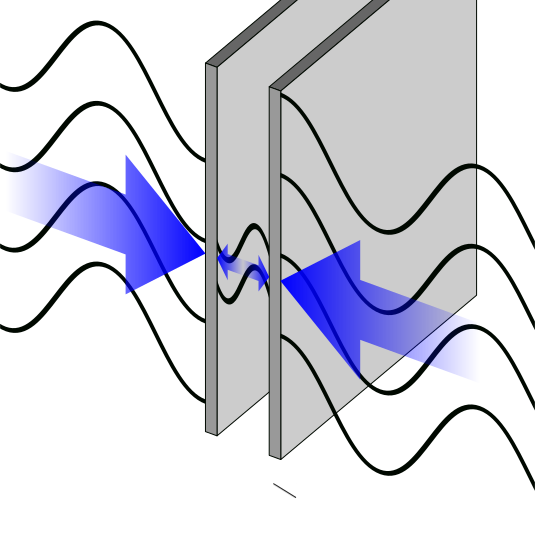
\includegraphics[width=.4\linewidth]{figs/Casimir-plates.pdf}
\caption{Силы Казимира, действующие на идеально проводящие пластины.}
\label{fig:plates}
\end{figure}

Обсудим еще один способ описать эффект Казимира в нашей системе. 
Каждая волна, как известно, оказывает давление на пластину. 
Чем ближе находятся пластины, тем меньше волн между ними может существовать, и тем слабее они будут расталкиваться. 
В то же время, пространство снаружи ничем не ограничено, волн в нем может существовать существенно больше, чем между пластинами. 
То есть снаружи на пластины действует сравнительно большая сближающая сила. 
Эта ситуация проиллюстрирована на рис.~\ref{fig:plates}. 
Выходит, что чем меньше расстояние между пластинами, тем сильнее они притягиваются. 
На практике это играет большую отрицательную роль в системах с размерами порядка долей микрометра и меньше, поскольку детали наномеханизмов попросту слипаются в комок. 

В общем случае эффект Казимира можно представить следующим образом. 
При помещении какого-либо объекта в вакуум квантовые флуктуации изменяются, поскольку поля должны удовлетворять определенным условиям на границе вакуум-вещество. 
Энергия системы зависит от формы объекта, а значит, имеется какая-то сила. 
Существенно и удачно то, что эта сила не всегда притягивающая~\cite{General.van-der-Waals}. 
Например, идеально проводящая незаряженная сфера расталкивается изнутри за счет квантовых флуктуаций~\cite{SphericalShell}. 

%%%%%%%%%%%%%%%%%%%%%%%%%%%%%%%%%%%%%%%%
\subsection{Отталкивающие силы Казимира}

\begin{figure}
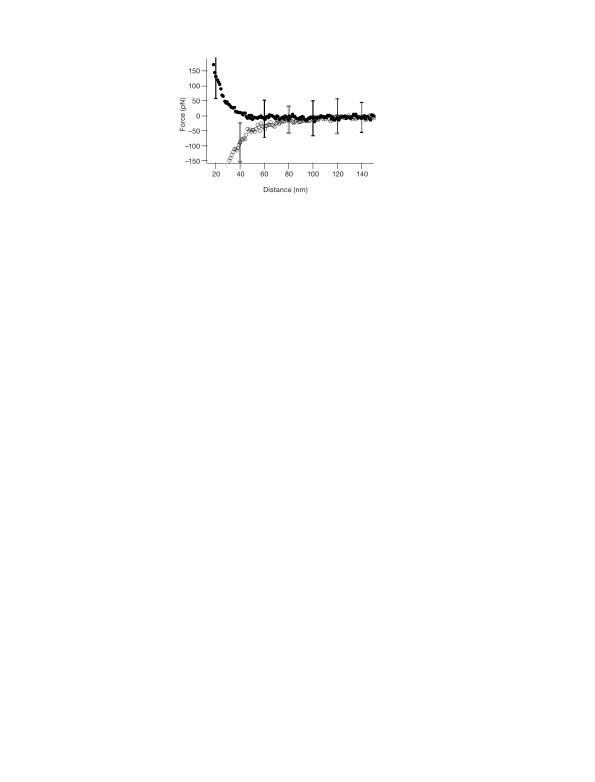
\includegraphics[width=.5\linewidth]{figs/Repulsive-graph}
\caption{Голубые (оранжевые) кружки показывают силу между золотой сферой и пластинкой из диоксида кремния (золота) в бромбензоле.}
\label{fig:rep.graph}
\end{figure}

Тема отталкивающих сил Казимира привлекает большое внимание из-за возможности применения в технологиях во-первых для достижения сверхнизкого трения, а во-вторых для избавления от упомянутых неприятностей, связанных с притягивающей силой. 
Экспериментально отталкивание наблюдалось лишь в одной конфигурации -- между двумя диэлектриками с разными проницаемостями, разделенными жидкостью с промежуточным значением проницаемости~\cite{Repulsion.firstexp}. Величина отталкивающей силы между золотом и диоксидом кремния в бромбензоле сравнима с притяжением между двумя золотыми телами, как видно на рис.~\ref{fig:rep.graph}. Вместо двух плоских пластин в эксперименте использовались пластина и сфера, поскольку расположить пластины параллельно на таком расстоянии сложно, а сфера достаточно близка к параллельной плоскости. 

Теоретически были найдены многие подходящие системы, включая идеальные электрический и магнитный проводники~\cite{Repulsion.magnetic}, метаматериалы~\cite{Repulsion.metamaterial}. 
Однако все упомянутое довольно сложно применить на практике. 
Успехом было обнаружение отталкивания в системах с обычными проводниками: эллиптической металлической частицей и проводящей поверхностью с дыркой~\cite{Repulsion.aperture}, полубесконечными плоскостями, плоскостью и иголкой~\cite{Repulsion.plates.needle}, анизотропно поляризуемыми атомами и различными поверхностями~\cite{Repulsion.conductors}. 

\begin{figure}[b!]
\includegraphics[width=.5\linewidth]{figs/Chiral-Casimir-new}
\caption{Отношение сил Казимира между проводящими пластинами в хиральной среде $F_C$ и в вакууме $F_0$ в зависимости от расстояния между ними для двух значений внешнего магнитного поля.}
\label{fig:Chiral.Casimir}
\end{figure}

В общем случае было доказано, что в системах незаряженных симметрично расположенных проводников невозможно реализовать отталкивающие силы Казимира~\cite{Casimir.attr.theorem}. 
Однако этот результат основывается на отсутствии как внешних сил, так и оптической активности материалов. 
Неудивительно, что искать новые явления приходится среди специфически ведущих себя веществ. 
Совсем недавно был найден способ добиться отталкивания в хиральной среде (в которой скорости распространения лево- и правополяризованных волн не совпадают)~\cite{Repulsion.tunable}. 
Более того, вводя внешнее магнитное поле в такой системе, можно переходить от притяжения к отталкиванию, то есть, потенциально, подстраивать силу Казимира под собственные нужды. 
Необходимо, однако, заметить, что требуемые для таких манипуляций поля могут оказаться очень большими. 
Тем не менее, достичь равновесия относительно сил Казимира можно и за счет одной лишь хиральной среды, поскольку из-за нее сила существенно зависит от расстояния между объектами, как показано на рис.~\ref{fig:Chiral.Casimir}, где $F_0 = -{\pi^2\hbar c}/{(240\,l^4)}$ -- поверхностная сила между идеально проводящими пластинами в вакууме. 
Участки с $F_C/F_0<0$ соответствуют отталкиванию. 
Как видно, существуют и устойчивые точки равновесия. 



\subsection{Заключение}

Изучение, казалось бы, простой из-за пустоты среды существенно осложняется квантовыми эффектами, которые находят подтверждение в эксперименте. 
Относящиеся к изложенным темам вакуумы квантовой электродинамики и квантовой хромодинамики не являются единственными.
Все взаимодействия могут привести к образованию виртуальных частиц, а значит, и квантовым флуктуациям. 
Фундаментальным теоретическим вопросом уже много лет остаются гравитационные квантовые флуктуации, предположительно приводящие к флуктуациям метрики пространства-времени, ее нелокальности и образованию виртуальных черных дыр. 

Очередной загадкой квантовых флуктуаций является энергия вакуума, которая должна присутствовать в общей теории относительности в уравнениях Эйнштейна в виде космологической постоянной. 
Проблема заключается в том, что, согласно даже самым оптимистичным современным представлениям, включающим до сих пор не нашедшую подтверждения суперсимметрию, ее теоретическое значение на 60 порядков больше экспериментального. 

С практической точки зрения, использование энергии вакуума может предоставить технологии совершенно нового уровня. Но поиск и реализация способных на такое устройств чрезвычайно сложны. Несмотря на все прилагаемые усилия на протяжении многих десятилетий, отталкивающие силы до сих пор экспериментально наблюдались лишь в одном типе систем. 





%%%%%%%%%%%%%%%%
%% References %%
%%%%%%%%%%%%%%%%
\begin{thebibliography}{99}
\bibitem{electron.g-2.exp} 
	\bibauthor{D. Hanneke, S. Fogwell Hoogerheide, and G. Gabrielse}, 
	\bibtitle{Cavity control of a single-electron quantum cyclotron: Measuring the electron magnetic moment}, 
	\href{http://dx.doi.org/10.1103/PhysRevA.83.052122}{Phys. Rev. A \textbf{83}, 052122 (2011)}.

\bibitem{electron.g-2.theory}
	\bibauthor{T. Aoyama \textit{et al}},
	\bibtitle{Tenth-order electron anomalous magnetic moment: Contribution
of diagrams without closed lepton loops}, 
	\href{http://dx.doi.org/10.1103/PhysRevD.91.033006}{Phys. Rev. D 91, 033006 (2015)}.

\bibitem{LambShift.exp}
	\bibauthor{W. E. Lamb and R. C. Retherford}, 
	\bibtitle{Fine Structure of the Hydrogen Atom by a Microwave Method}, 
	\href{http://dx.doi.org/10.1103/PhysRev.72.241}{Phys. Rev. 72, 241 (1947)}.

\bibitem{Hawking}
	\bibauthor{S. W. Hawking}, 
	\bibtitle{Black hole explosions?}, 
	\href{http://dx.doi.org/10.1038/248030a0}{Nature 248, 30 (1974)}.

\bibitem{Casimir.van-der-Waals}
	\bibauthor{H. B. G. Casimir and D. Polder}, 
	\bibtitle{The Influence of Retardation on the London-van der Waals Forces}, 
	\href{http://dx.doi.org/10.1103/PhysRev.73.360}{Phys. Rev. 73, 360 (1948)}.

\bibitem{Casimir.vacuum}
	\bibauthor{H. B. G. Casimir}, 
	\bibtitle{On the Attraction Between Two Perfectly Conducting Plates}, 
	Kon.Ned. Akad. Wetensch. Proc. 51, 793 (1948).

\bibitem{General.van-der-Waals}
	\bibauthor{И. Е. Дзялошинский, Е. М. Лифшиц и Л. П. Питаевский}, 
	\bibtitle{Общая теория ван-дер-Ваальсовых сил}, 
	\href{http://dx.doi.org/10.3367/UFNr.0073.196103b.0381}{Усп. физ. наук 73, 381 (1961)}.

\bibitem{SphericalShell}
	\bibauthor{T. H. Boyer}, 
	\bibtitle{Quantum Electromagnetic Zero-Point Energy of a Conducting Spherical Shell and the Casimir Model for a Charged Particle}, 
	\href{http://dx.doi.org/10.1103/PhysRev.174.1764}{Phys. Rev. 174, 1764 (1968)}.

\bibitem{Repulsion.firstexp}
	\bibauthor{J. N. Munday, F. Capasso, and V. A. Parsegian}, 
	\bibtitle{Measured long-range repulsive Casimir-Lifshitz forces}, 
	\href{http://dx.doi.org/10.1038/nature07610}{Nature 457, 170 (2009)}.

\bibitem{Repulsion.magnetic}
	\bibauthor{T. H. Boyer}, 
	\bibtitle{Van der Waals forces and zero-point energy for dielectric and permeable materials}, 
	\href{http://dx.doi.org/10.1103/PhysRevA.9.2078}{Phys. Rev. A 9, 2078 (1974)}.

\bibitem{Repulsion.metamaterial}
	\bibauthor{A. P. McCauley \textit{et al.}}, 
	\bibtitle{Microstructure effects for Casimir forces in chiral metamaterials}, 
	\href{http://dx.doi.org/10.1103/PhysRevB.82.165108}{Phys. Rev. B 82, 165108 (2010)}.

\bibitem{Repulsion.aperture}
	\bibauthor{M. Levin \textit{et al.}}, 
	\bibtitle{Casimir Repulsion between Metallic Objects in Vacuum}, 
	\href{http://dx.doi.org/10.1103/PhysRevLett.105.090403}{Phys. Rev. Lett. 105, 090403 (2010)}.

\bibitem{Repulsion.plates.needle}
	\bibauthor{K. A. Milton \textit{et al.}}, 
	\bibtitle{Casimir-Polder repulsion near edges: Wedge apex and a screen with an aperture}, 
	\href{http://dx.doi.org/10.1103/PhysRevA.83.062507}{Phys. Rev. A 83, 062507 (2011)}.

\bibitem{Repulsion.conductors}
	\bibauthor{K. A. Milton \textit{et al.}}, 
	\bibtitle{Casimir-Polder repulsion: Polarizable atoms, cylinders, spheres, and ellipsoids}, 
	\href{http://dx.doi.org/10.1103/PhysRevD.85.025008}{Phys. Rev. D 85, 025008 (2012)}.

\bibitem{Casimir.attr.theorem}
	\bibauthor{O. Kenneth and I. Klich}, 
	\bibtitle{Opposites Attract: A Theorem about the Casimir Force}, 
	\href{http://dx.doi.org/10.1103/PhysRevLett.97.160401}{Phys. Rev. Lett. 97, 160401 (2006)}.

\bibitem{Repulsion.tunable}
	\bibauthor{Q.-D. Jiang and F. Wilczek}, 
	\bibtitle{Chiral Casimir forces: Repulsive, enhanced, tunable},
	\href{http://dx.doi.org/10.1103/PhysRevB.99.125403}{Phys. Rev. B 99, 125403 (2019)}.
\end{thebibliography}


\end{document}
%%%%%%%%%%%%%%%%%%%
%% Document ends %%
%%%%%%%%%%%%%%%%%%%

